%  article.tex (Version 3.3, released 19 January 2008)
%  Article to demonstrate format for SPIE Proceedings
%  Special instructions are included in this file after the
%  symbol %>>>>
%  Numerous commands are commented out, but included to show how
%  to effect various options, e.g., to print page numbers, etc.
%  This LaTeX source file is composed for LaTeX2e.

%  The following commands have been added in the SPIE class 
%  file (spie.cls) and will not be understood in other classes:
%  \supit{}, \authorinfo{}, \skiplinehalf, \keywords{}
%  The bibliography style file is called spiebib.bst, 
%  which replaces the standard style unstr.bst.  

%%\documentclass[]{spie}  %>>> use for US letter paper
\documentclass[a4papert,12pt]{spie}  %>>> use this instead for A4 paper
%%\documentclass[nocompress]{spie}  %>>> to avoid compression of citations
%% \addtolength{\voffset}{9mm}   %>>> moves text field down
%% \renewcommand{\baselinestretch}{1.65}   %>>> 1.65 for double spacing, 1.25 for 1.5 spacing 
%  The following command loads a graphics package to include images 
%  in the document. It may be necessary to specify a DVI driver option,
%  e.g., [dvips], but that may be inappropriate for some LaTeX 
%  installations. 
\usepackage[]{graphicx}
\usepackage[sort, numbers]{natbib}
\usepackage{hyperref}
\usepackage{adjustbox,lipsum}
\graphicspath{ {/Users/anirudhnair/code/GeoSched/src/GoogleTrace/plots} }
\usepackage{subfig}
\usepackage[margin=0.5in]{geometry}

\title{GeoSched: Minimizing Cost of Cloud Workloads in Geo-Distributed Data Centers} 
\author{Anirudh Jayakumar and Harshit Dokania \\
University of Illinois at Urbana-Champaign \\
\{ajayaku2,hdokani2\}@illinois.edu 
}

\newenvironment{list1}{
  \begin{list}{\ding{113}}{%
      \setlength{\itemsep}{0in}
      \setlength{\parsep}{0in} \setlength{\parskip}{0in}
      \setlength{\topsep}{0in} \setlength{\partopsep}{0in}
      \setlength{\leftmargin}{0.17in}}}{\end{list}}
\newenvironment{list2}{
  \begin{list}{$\bullet$}{%
      \setlength{\itemsep}{0in}
      \setlength{\parsep}{0in} \setlength{\parskip}{0in}
      \setlength{\topsep}{0in} \setlength{\partopsep}{0in}
      \setlength{\leftmargin}{0.2in}}}{\end{list}}
 

%%%%%%%%%%%%%%%%%%%%%%%%%%%%%%%%%%%%%%%%%%%%%%%%%%%%%%%%%%%%% 
%>>>> uncomment following for page numbers
% \pagestyle{plain}    
%>>>> uncomment following to start page numbering at 301 
%\setcounter{page}{301} 
 
  \begin{document} 
  \maketitle 

%%%%%%%%%%%%%%%%%%%%%%%%%%%%%%%%%%%%%%%%%%%%%%%%%%%%%%%%%%%%% 
\begin{abstract}
Today, many of the leading cloud service providers have geographically distributed data centers to serve millions of users around the world. The need for a geo-distributed data center arising from the need to provide low-latency and  high-availability of the different services. The workloads that run on these data centers are also highly varied. A typical data centers run jobs of different kinds including business-critical workloads---web servers, mail servers, instant messaging services etc, big-data processing, real-time data analytics and HPC jobs. As cloud services grow to serve more customers, there is an increasing need for a workload provisioning mechanism which can minimize the cost of operation of the data center while still obeying the SLA and also minimizing the user-perceived latency. 

We present GeoSched, a job provisioning framework that is workload aware, energy-aware and cooling-aware. GeoSched considers the workload type (batch process, real-time processing, web-service), the energy source of the data center (brown and green energy), electricity pricing of the region, cooling techniques used in the data center (air economizer) and also the history of jobs to predict the load patterns and cluster utilization. We wish to evaluate GeoSched on industry workload traces and also on synthetic workloads that can mimic the real-world data center workload. 
\end{abstract}


%%%%%%%%%%%%%%%%%%%%%%%%%%%%%%%%%%%%%%%%%%%%%%%%%%%%%%%%%%%%%
\section{Related Work}
\label{sec:intro}  % \label{} allows reference to this section
Cost minimization has been extensively studied both in the context of a single data center and a geo-distributed data center. Most of the work has been targeted towards minimizing the energy consumption of the data center to reduce the operational cost. For example, the work by Gu et al. \cite{gu2014cost} studies the influence of task assignment, data placement  and data movement on the operational expenditure of large-scale geo-distributed data centers for big data applications. The authors jointly optimize  these three factors by proposing a 2-D Markov chain to derive the average task completion time and solve the model as a MILP problem. On similar lines Agarwal et al. \cite{agarwal2010volley} propose an automated data placement mechanism Volley for geo-distributed cloud services with the consideration of WAN bandwidth cost, data center capacity limits, data inter-dependencies, etc. 

Yu et all.\cite{yu2015energy} propose minimizing energy cost for distributed Internet data centers (IDCs) in smart microgrids by considering system dynamics like uncertainties in electricity price, workload, renewable energy generation, and power outage state. They model the problem as a stochastic program and solve it using Lyapunov optimization technique. The work by Ren and He  \cite{ren2013coca} propose an online algorithm, called COCA to minimize data center operational cost while satisfying carbon neutrality. Unlike some of the existing research, COCA enables distributed server-level resource management: each server autonomously adjusts its processing speed and optimally decides the amount of workloads to process. This work is restricted to a single data center with heterogeneous resources. 

Cooling energy is a substantial part of the total energy spent by a data center. According to some reports, this can be as high as 50\% \cite{sullivan2002alternating}, \cite{patel2003smart},\cite{sawyer2004calculating} of the total energy budget. There has been a lot of work both at the application/middleware level \cite{TempLDBSC11}, \cite{leverich2010energy} as well as provisioning techniques  \cite{tang2007thermal}, \cite{chen2010integrated} that try to minimize the cooling energy. Li et all. \cite{li2014coordinating} proposes SmartCool, a power optimization scheme that effectively coordinates different cooling techniques and dynamically manages workload allocation for jointly optimized cooling and server power. Unlike existing work that addresses different cooling techniques in an isolated manner, SmartCool integrates different cooling systems as a constrained optimization problem. Also, since geo-distributed data centers have different ambient temperatures, SmartCool dynamically dispatches the incoming requests among a network of data centers with heterogeneous cooling systems to best leverage the high efficiency of free cooling.  

\iffalse


Other research related to cooling efficiency include the work by Liu et all \cite{liu2012renewable}  that reduces electricity cost and environmental impact using a holistic approach that integrates renewable supply, dynamic pricing, and cooling supply including chiller and outside air cooling, with IT workload planning to improve the overall sustainability of data center operations. The authors first predict renewable energy as well as IT demand. Then they use these predictions to generate an IT workload management plan that schedules IT workload and allocates IT resources within a data center according to time varying power supply and cooling efficiency. Pakbaznia and Pedram \cite{pakbaznia2009minimizing} focuses on minimizing power for both IT equipment and air conditioning power usage. The authors consider both server consolidation and task assignment together and formulate the resulting optimization problem a a ILP problem and present a heuristic algorithm that loves it in polynomial time.

There are also research done to look at the impact of failures in data centers on the operational cost. The work by Cui et al. \cite{cui2014shadows} considers the increase in energy consumption due to failures in large scale clouds. A slower shadow replication of the main process is used to recover from faults thereby saving energy upto 30\%. Guenter et al. \cite{guenter2011managing} also considers different trade-offs between cost, performance and reliability to formulate an optimization problem that minimizes energy costs, reliability costs and unmet demands. VM migration techniques are also used extensively to increase the energy efficiency of cloud data centers. One such approach is proposed by Rodero et al. \cite{rodero2012energy} where the author  propose to use applications��s profiling (CPU, memory, bandwidth) to  design application-centric energy-aware strategy for VM allocation during VM migration.

Researchers have also studied the efficient use of green energy in data centers. Goiri et al. \cite{goiri2011greenslot} propose a system GreenSlot that maximizes the use of green energy available at data centers while ensuring all job deadlines are met. GreenSlot predicts the solar energy available in data centers in near future and schedules the workload to maximize green energy consumption and meeting jobs��s deadlines. Green- Slot can increase green energy consumption by up to 117\% and decrease energy cost by up to 39\%, compared to a conventional scheduler. 



%%%%%%%%%%%%%%%%%%%%%%%%%%%%%%%%%%%%%%%%%%%%%%%%%%%%%%%%%%%%%
\section{Problem Statement} 

Minimize the total cost of operations of a geo-distributed data center running cloud workloads by minimizing the energy costs subject to business constraints like the service level agreement(SLA) and other technical constraints like data center capacity limits. The energy costs will depend on the power usage of the IT infrastructure and also the energy required by the cooling infrastructure to maintain the desired temperature inside the data center. Additionally, the solution should also consider the different energy source(green and brown) available at the data center and the different workload types that are typical to a cloud data center.

%%%%%%%%%%%%%%%%%%%%%%%%%%%%%%%%%%%%%%%%%%%%%%%%%%%%%%%%%%%%%
\fi

\section{Cloud Workload } 
With the increase in the adoption of cloud computing by businesses around the world, more and more workloads are moving out of traditional data centers into the cloud. A cloud data center typically handles a range of IT workloads. These workloads include service-critical and latency sensitive interactive applications that run 24x7 such as instant messengers, e-mail applications and other internet services, and batch-style applications such as scientific HPC applications, BigData applications like financial analysis and MapReduce applications. A thoughtful management of these workloads are necessary not only to provide customers with low-latency services but also to reduce the energy consumption of the data centers that run these workloads. A good way to study these workloads are by analyzing real-world or synthetic workload traces. We look at workload traces in detail in section \ref{traces} and \ref{googletrace}

\subsection{Workload Traces} \label{traces}
Unfortunately, there is a lack of real-world traces in the cloud computing research community. As a result, there are limited work done to understand the diversity in cloud workloads. The first large-scale workload trace was released by Google in 2011\cite{googletracedata}, featuring traces from over 12,000 servers over a period of 29 days. Various studies have been carried out to understand the characteristic of the Google trace data. Other real-world traces include Wikipedia request trace \cite{urdaneta2009wikipedia} and Hadoop logs from Yahoo! \cite{yahootrace}There have also been attempts to generate synthetic workload traces using known real-world workload characteristics \cite{beitch2010rain} \cite{wang2011towards}. For the sake of this work, we have decided to use the workload trace from Google. 

\subsection{Custom Trace Format}
To have a common trace format to represent different real-world and synthetic workload traces, we have formulated a trace format similar to standard workload format (swf) \cite{chapin1999benchmarks} defined for grid and supercomputing traces. Table \ref{tab:format} provides information about each field int the trace format.
 
\begin {table}[ht]
\caption {Trace format description} \label{tab:format} 
 \scalebox{0.9}{\begin{tabular}{ | p{4cm} |l  |p{11 cm}|  }
    \hline
    \bf{Field Name} & \bf{Type} & \bf{Description}   \\ \hline
     JobID & INTEGER  & Unique job identifier for each job\\ \hline
     Arrival Time & INTEGER & Arrival time in microseconds \\ \hline
     Scheduled Time & INTEGER  & Arrival time in microseconds\\ \hline
     Finish Time & INTEGER  & Arrival time in microseconds\\ \hline
     Schedule class & INTEGER  & Latency class of the job. \\ \hline
     Tasks & INTEGER  & Total number of tasks in the job. \\ \hline
     Total CPU& INTEGER  & Aggregate sum of CPU used by all the tasks in the job\\ \hline
     Total Memory& INTEGER   & Aggregate sum of memory used by all the tasks in the job \\ \hline
     User& INTEGER  & Unique user identifier \\ \hline
     SLA Param1&  FLOAT & SLA parameter placeholder\\ \hline
     SLA Param2&  FLOAT & SLA parameter placeholder\\ \hline
     SLA Param3&  FLOAT & SLA parameter placeholder\\ \hline
    \end{tabular}}
\end{table}

\subsection{Google Workload Trace} \label{googletrace}
Google trace has job and task information in different files. We consolidated all the required information and generated a single work trace file with the format described in the previous section. For our work, we model five different data centers located at different parts of the globe. A detailed explanation about the data center profile are given in section \ref{sec:datacenter}. To simulate workload execution in these five data centers we have extracted five set of traces each worth five days of incoming workload from the original google trace. So, this covers 25 days of traces out of the 29 available days. We label these 5 set of traces from A to E. Additionally, in our experiments we wish to only consider those jobs that end without any failures. Therefore, we clean the original traces by removing all jobs that is either failed or get killed. 

\begin{figure}[ht] 
\centering
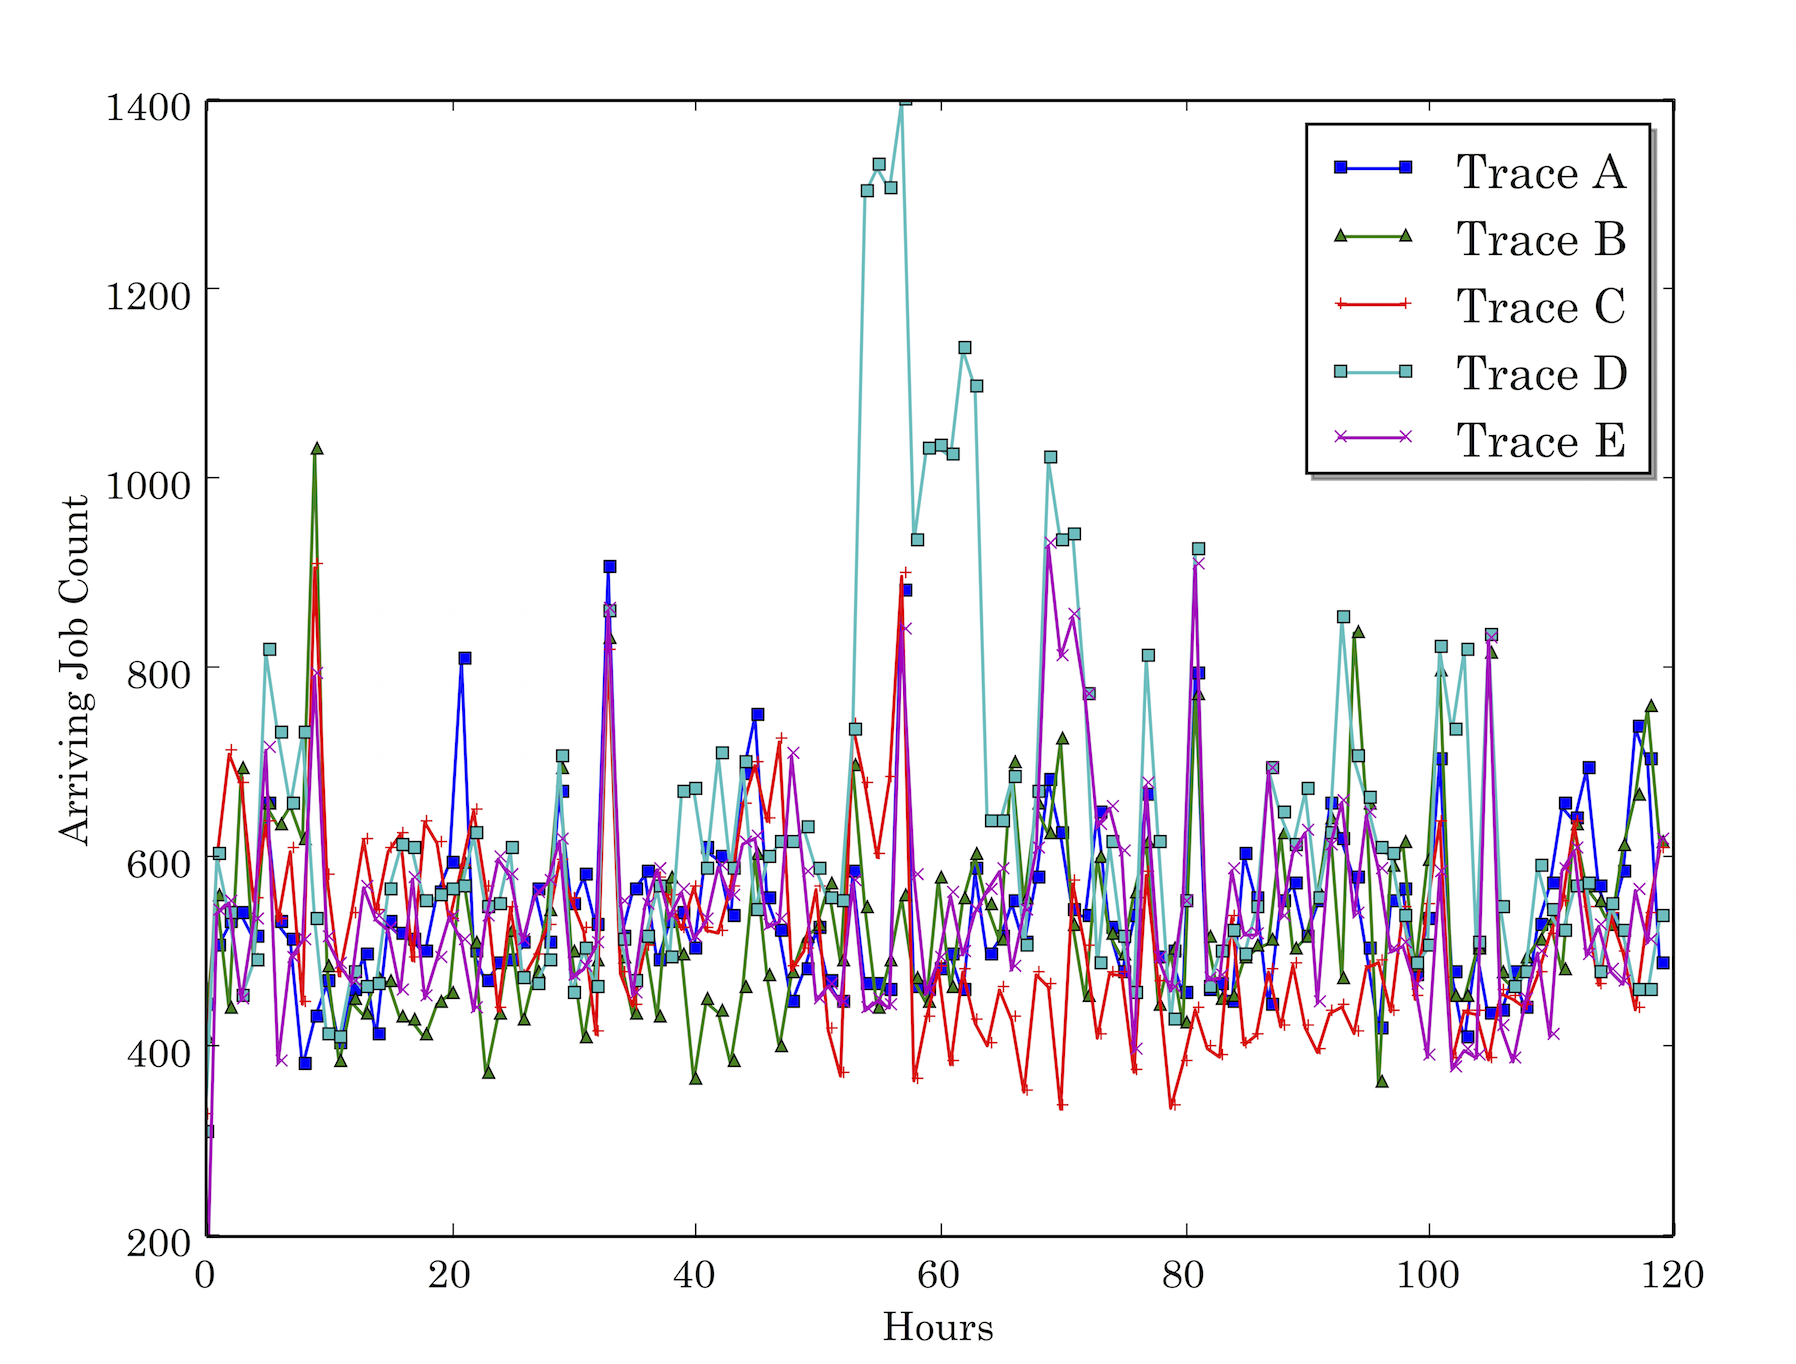
\includegraphics[scale=0.40]{arrivalrate.png}
\caption{Arrival rate of jobs }
\label{fig:arrivalrate}
\end{figure}

Now we will look at some characteristics of the traces. Table \ref{tab:tracestat} describes the statistics for each of the five traces grouped by the scheduling class of the job. In google traces, CPU and memory usage are normalized relative to the largest capacity of the resource on any machine in the trace (which is 1.0). Most of the class 0 and class 2 jobs are batch jobs with less latency requirements. Generally, these are the kind of jobs that can be provisioned on other data centers as their deadlines are not strict.  You will find that as the sensitivity increases the running time of these jobs also increase. High-sensitive jobs are generally service jobs and run of longer periods of time. Figure \ref{fig:pie} shows a pie chart of the job counts in different schedule classes for all the 5 traces. You will notice that the job count for class 3 (high latency-sensitivity) jobs are low. This is because these jobs generally run for long period of time, typically months. Since we only consider jobs that start and end within the 29 day range such jobs are missed out in our traces. For our work, we will consider class-0 and class-1 jobs as candidates for optimizing the provisioning. We leave, class-2 and class-3 jobs to run on the data center where the job arrived since these are high-sensitive and their SLA demands will be strict.


\begin{figure}[]
\centering
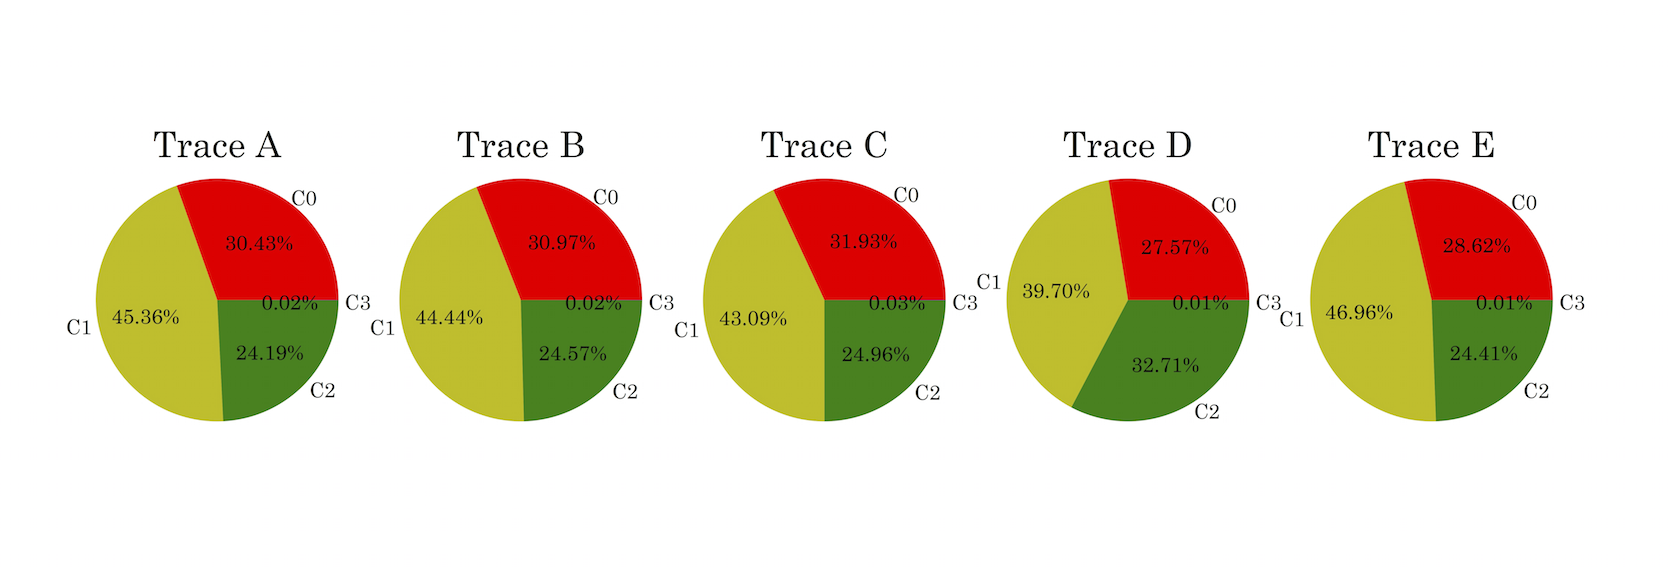
\includegraphics[scale=0.65]{pie}
\caption{ Distribution of job count in various schedule classes}
 \label{fig:pie}
\end{figure}

\begin{table}
\caption {Trace set statistics} \label{tab:tracestat} 
\adjustbox{max width=1\textwidth}{

\begin{tabular}{|l|l|l|l|l|l|l|l|l|l|l|l|l|l|l|l|}
\hline
 & \multicolumn{3}{l|}{\bf{Trace A}} & \multicolumn{3}{l|}{\bf{Trace B}} & \multicolumn{3}{l|}{\bf{Trace C}} & \multicolumn{3}{l|}{\bf{Trace D}} & \multicolumn{3}{l|}{\bf{Trace E}} \\ \hline
\textbf{\begin{tabular}[c]{@{}l@{}}Sched\\ Class\end{tabular}} & \textbf{\begin{tabular}[c]{@{}l@{}}Avg \\ CPU\end{tabular}} & \textbf{\begin{tabular}[c]{@{}l@{}}Avg\\ Mem\end{tabular}} & \textbf{\begin{tabular}[c]{@{}l@{}}RT\\  (secs)\end{tabular}} & \textbf{\begin{tabular}[c]{@{}l@{}}Avg\\ CPU\end{tabular}} & \textbf{\begin{tabular}[c]{@{}l@{}}Avg\\ Mem\end{tabular}} & \textbf{\begin{tabular}[c]{@{}l@{}}RT\\  (secs)\end{tabular}} & \textbf{\begin{tabular}[c]{@{}l@{}}Avg\\ CPU\end{tabular}} & \textbf{\begin{tabular}[c]{@{}l@{}}Avg\\ Mem\end{tabular}} & \textbf{\begin{tabular}[c]{@{}l@{}}RT\\  (secs)\end{tabular}} & \textbf{\begin{tabular}[c]{@{}l@{}}Avg\\ CPU\end{tabular}} & \textbf{\begin{tabular}[c]{@{}l@{}}Avg\\ Mem\end{tabular}} & \textbf{\begin{tabular}[c]{@{}l@{}}RT\\  (secs)\end{tabular}} & \textbf{\begin{tabular}[c]{@{}l@{}}Avg\\ CPU\end{tabular}} & \textbf{\begin{tabular}[c]{@{}l@{}}Avg\\ Mem\end{tabular}} & \textbf{\begin{tabular}[c]{@{}l@{}}RT\\  (secs)\end{tabular}} \\ \hline
0 & 0.075 & 0.051 & 415 & 0.123 & 0.096 & 345 & 0.083 & 0.065 & 385 & 0.093 & 0.092 & 373 & 0.093 & 0.074 & 333 \\ \hline
1 & 0.087 & 0.029 & 729 & 0.086 & 0.032 & 760 & 0.082 & 0.028 & 711 & 0.073 & 0.030 & 743 & 0.093 & 0.043 & 693 \\ \hline
2 & 0.067 & 0.043 & 1028 & 0.096 & 0.058 & 872 & 0.088 & 0.057 & 918 & 0.073 & 0.045 & 707 & 0.084 & 0.049 & 832 \\ \hline
3 & 0.088 & 0.12 & 1105 & 0.099 & 0.12 & 82 & 0.101 & 0.012 & 7961 & 0.081 & 0.051 & 17135 & 0.089 & 0.061 & 9021 \\ \hline
\end{tabular}
}
\end{table}

Figure \ref{fig:arrivalrate} shows the variation in job arrival for the traces. As you can see there is both intra-trace variation as well as inter-trace variation. This is representative of the real-world cloud workload pattern where bursty arrivals are common. There are opportunities to provision jobs to other data centers if the traffic at a particular data center is high. What is also important to notice is that the scheduling decision should be made quickly when the arrival rates of jobs are high, else there are chances for these jobs to miss the SLA. Hence, even the scheduler should be scalable during high volume traffic. 

Figure \ref{fig:runtime} shows the CDF of the job runtime. As you can see most of the jobs have runtime less than 1024 seconds. This pattern is consistent for all the trace sets. There are a few jobs that have higher run-times. As explained earlier, these jobs are primarily internet-service jobs that run for months. 


\begin{figure}[] 
\centering
\includegraphics[scale=0.40]{runtime}
\caption{CDF of the job duration}
\label{fig:runtime}
\end{figure}

In google workload trace, it is tough to study the resource usage since these value are scaled down and therefore and accurate picture of the resource utilization is tough to generate. In figure \ref{fig:resource} we can see that most jobs request a small portion of the cluster resources. Most of the resources in the google cluster are used by the few service jobs that are present. The large number of batch jobs only use a small percentage of the resources \cite{mishra2010towards} \cite{reiss2012heterogeneity}. From the above statistics, we believe that google workload trace provides an accurate representation of the real-world cloud datacenter workload.

\begin{figure} %
    \centering
    \subfloat[CPU resource ]{{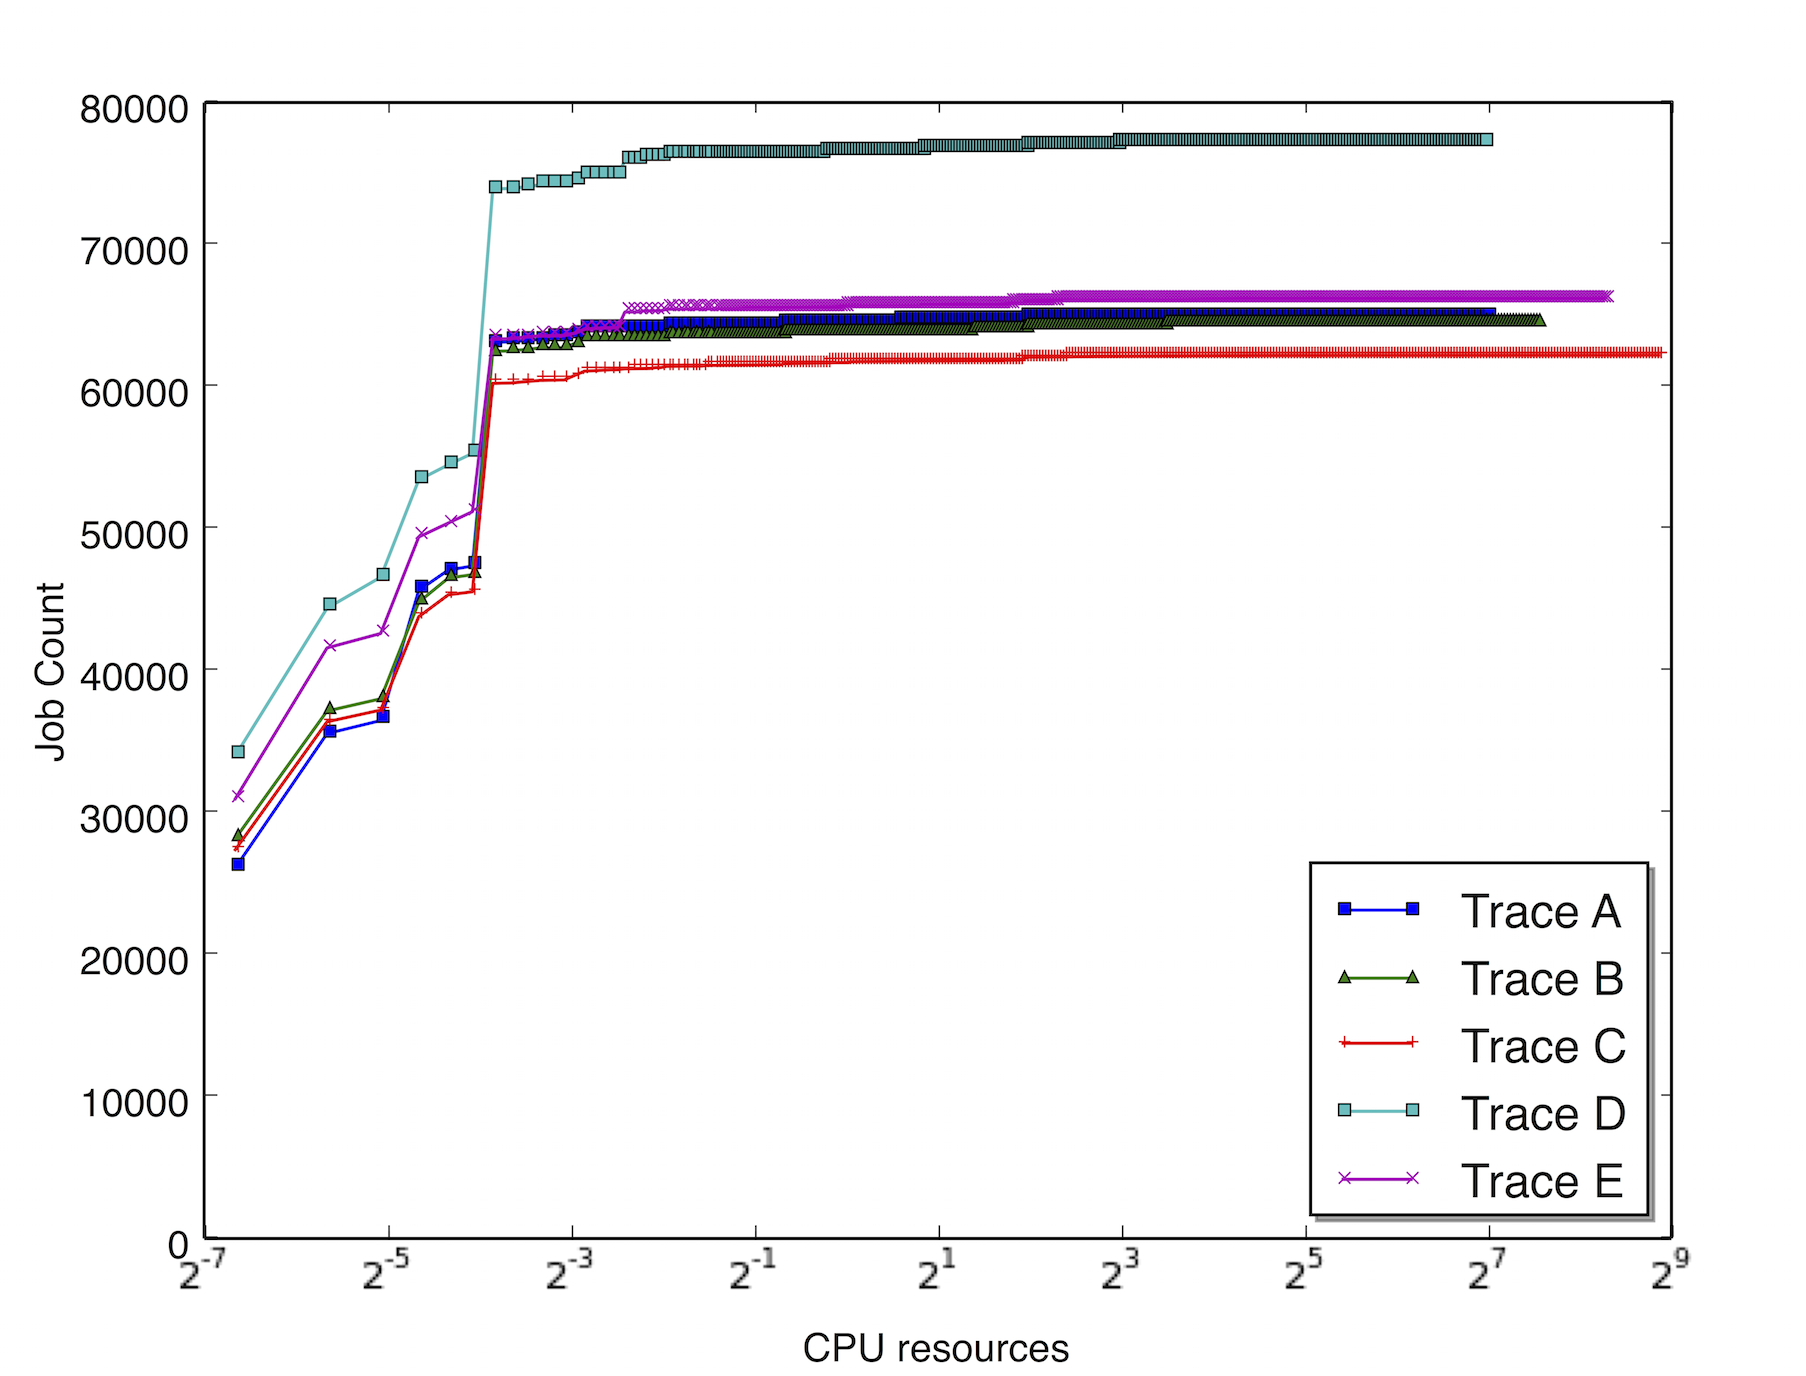
\includegraphics[width=9cm]{cpu} }}%
    \subfloat[RAM resource]{{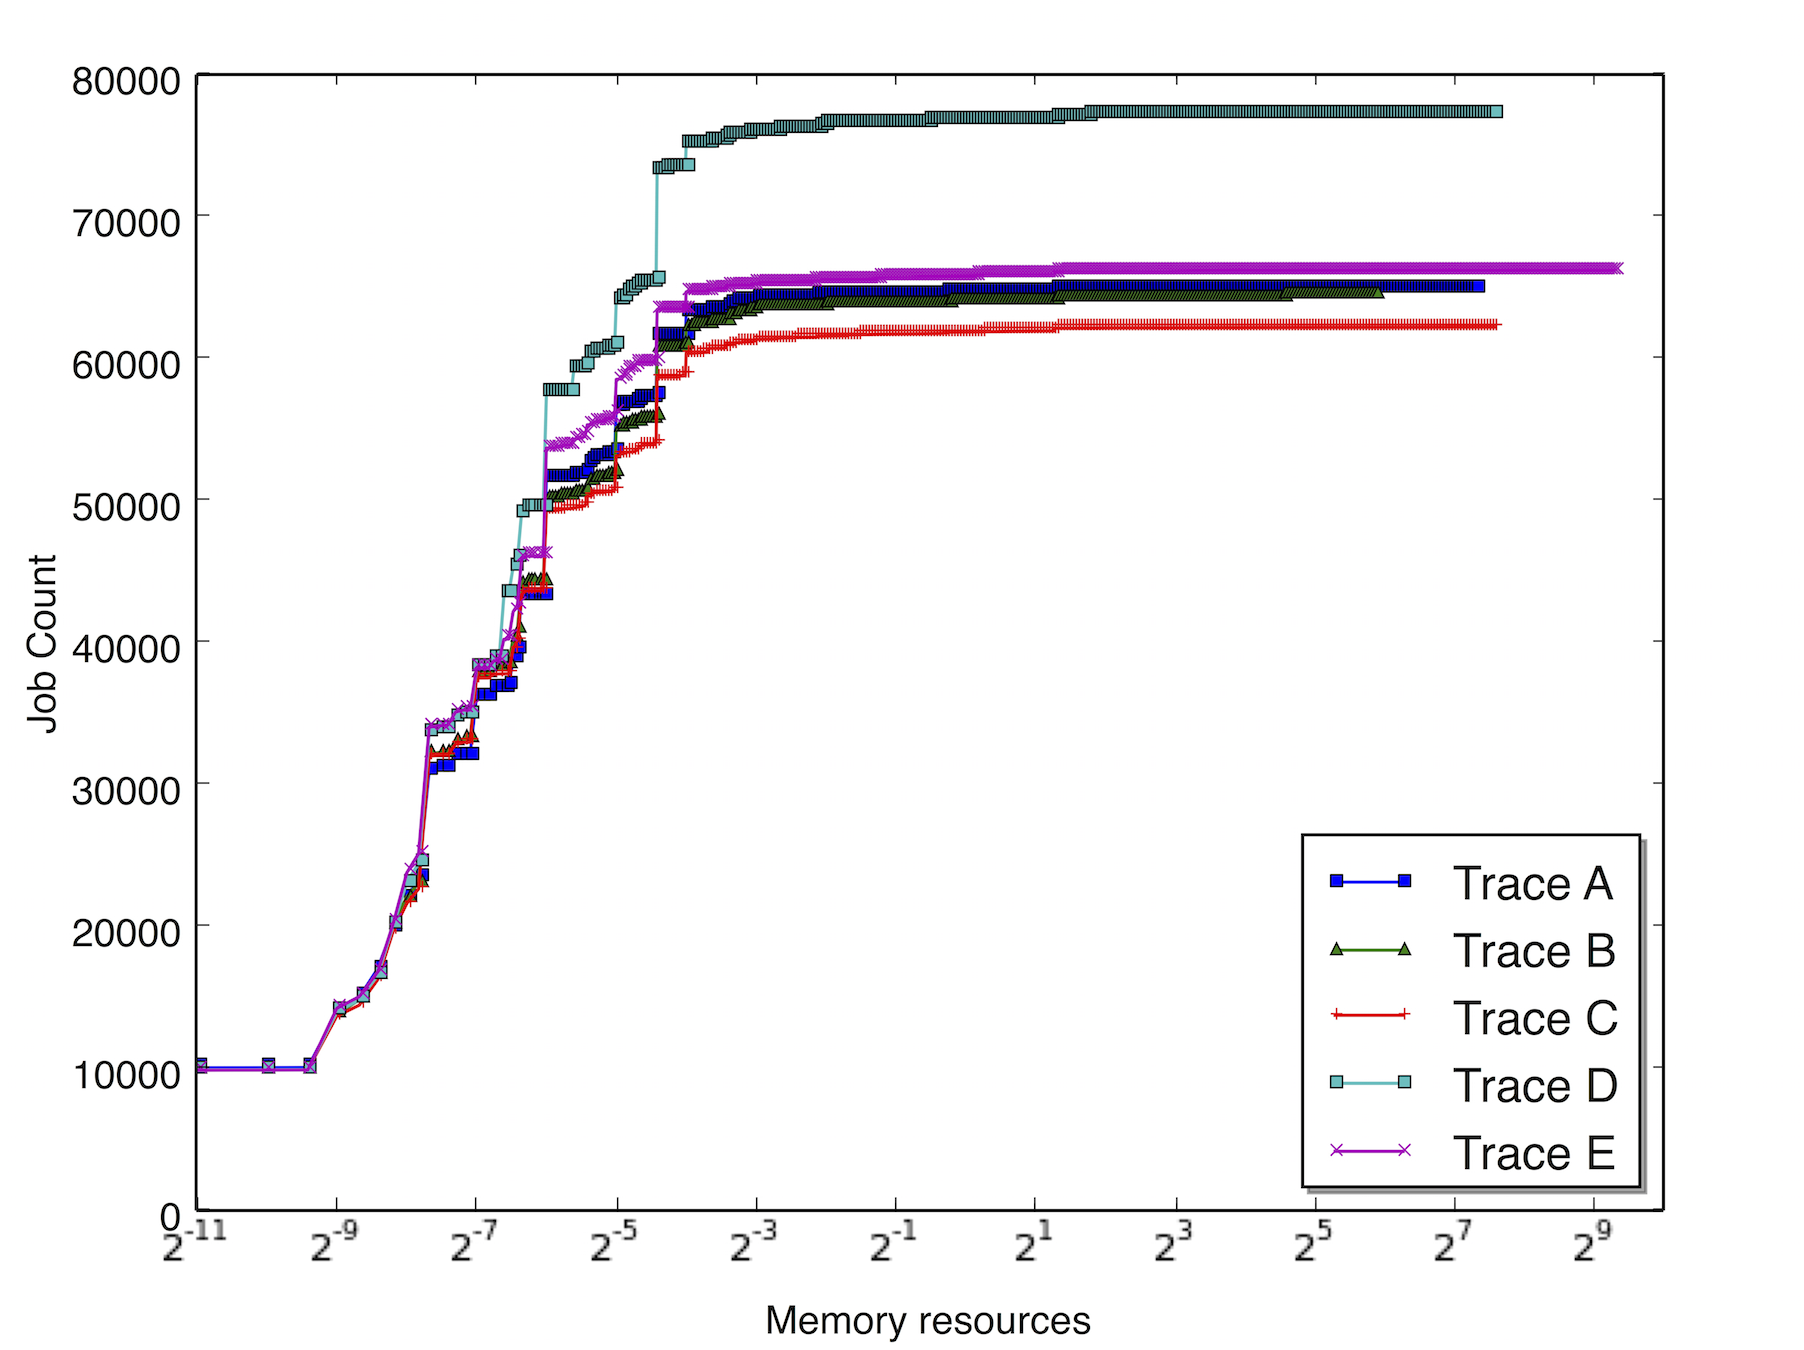
\includegraphics[width=9cm]{mem} }}%
    \caption{CDF of resource requested by jobs}%
    \label{fig:resource}%
\end{figure}

%%%%%%%%%%%%%%%%%%%%%%%%%%%%%%%%%%%%%%%%%%%%%%%%%%%%%%%%%%%%%

\section{Data Center Profiling } \label{sec:datacenter}

Provide some introduction about out profiling stratergy

\subsection{Geo-Distributed Data Center}

\subsection{Profile Parameters}
\subsubsection{Temperature}
\subsubsection{Electricity Pricing}
\subsubsection{Energy Source}

\subsection{Air Economizer}

%%%%%%%%%%%%%%%%%%%%%%%%%%%%%%%%%%%%%%%%%%%%%%%%%%%%%%%%%%%%%

\section{Scheduler simulator} 

Provide basic idea about our strategy

\subsection{Architecture}
Introduce cloudsim
\subsubsection{Components}
\subsubsection{Integration of traces and data center profile}
\subsubsection{Design}

%%%%%%%%%%%%%%%%%%%%%%%%%%%%%%%%%%%%%%%%%%%%%%%%%%%%%%%%%%%%%

\section{Scheduling Algorithm} 

Provide basic idea about our strategy

\subsection{Features considered}
\subsubsection{Energy Cost Model}
%\subsubsection{Optimization Techiques}
%\subsubsection{Design}

\section{ Milestones} 

    \begin{tabular}{ | p{4cm} |l  |p{11 cm}|  }
    \hline
    \bf{Item} & \bf{Deadline} & \bf{Description}   \\ \hline
    Study real-world and synthetic workloads & 10\textsuperscript{th} March  & We have started studying workloads traces for google cluster-data which provides traces from a 12k-machine cell for one month duration in May 2011.  \\ \hline
    Data Center profile & 20\textsuperscript{th} March  & In this process we will note the data center specific parameters such as electricity cost, available energy, economizer, cooling energy that is useful for simulating geo-distributed data centers. \\ \hline
    Simulator design and implementation& 12\textsuperscript{th} April  & Implement the simulator infrastructure for multi-datacenter environment.  \\ \hline
    Feature Extraction and Optimization & 25\textsuperscript{th} April  & Here we identifying all the necessary features that contribute to the energy cost  and build an optimization technique which is adaptive to workload characteristics and data center's resource capacity and electricity costs \\ \hline
    Evaluation & 7\textsuperscript{th} May  & This phase we will be simulating data centers with previously gathered data center profile and using the optimization technique mentioned above \\ \hline
    
    \end{tabular}


  

%%%%%%%%%%%%%%%%%%%%%%%%%%%%%%%%%%%%%%%%%%%%%%%%%%%%%%%%%%%%%


\bibliography{report}   %>>>> bibliography data in report.bib
\bibliographystyle{spiebib}   %>>>> makes bibtex use spiebib.bst

\end{document} 
